\section{Evaluation}

\subsection{Methodology}

We evaluate four network sizes, $N \in \{8, 12, 16, 20\}$, and four copy budgets, $K \in \{1, 2, 4, N\}$. The choice of $K{=}1$ provides a direct-delivery baseline, while $K{=}N$ represents an aggressive bounded-replication extreme. For every $(N,K)$ pair, we run 50 independent trials with different random seeds using the same encounter-rate and encounter-duration parameters. Each trial carries a single bundle from a fixed source to a fixed destination and runs until delivery or a timeout horizon of 60 simulated time units.

We report four metrics:
\begin{itemize}
    \item \textbf{Delivery rate}: fraction of trials in which the bundle reaches the destination.
    \item \textbf{Delay}: delivery latency, measured only over successful trials.
    \item \textbf{Data overhead}: average number of \texttt{SPRAY} and \texttt{DELIVER} transmissions.
    \item \textbf{Control overhead}: average number of summary exchanges.
\end{itemize}

All experiments are reproducible through the evaluation script \texttt{examples/evaluate\_spray\_wait.py}. The script writes the full CSV file and generates the figures included below. The exact experiment in this report can be regenerated with the command shown below.

\begin{figure}[t]
\begin{minipage}{\linewidth}
\small\ttfamily
python examples/evaluate\_spray\_wait.py --copies 1 2 4 N --trials 50
\end{minipage}
\caption{Command used to regenerate the reported results.}
\label{lst:repro}
\end{figure}

\subsection{Main Results}

Table~\ref{tab:delivery} summarizes delivery probability. The first clear pattern is that delivery becomes harder as the network grows when the copy budget is small. With $K{=}1$, delivery falls from 90\% at 8 nodes to 38\% at 20 nodes. In contrast, $K{=}N$ achieves 100\% delivery for all tested sizes. Even moderate replication helps substantially: at 20 nodes, increasing the budget from $K{=}1$ to $K{=}4$ nearly doubles delivery probability, from 38\% to 74\%.

\begin{table}[t]
    \centering
    \caption{Delivery rate over 50 trials per setting.}
    \label{tab:delivery}
    \begin{tabular}{ccccc}
        \hline
        Nodes & $K{=}1$ & $K{=}2$ & $K{=}4$ & $K{=}N$ \\
        \hline
        8  & 0.90 & 0.98 & 1.00 & 1.00 \\
        12 & 0.72 & 0.96 & 1.00 & 1.00 \\
        16 & 0.50 & 0.74 & 0.92 & 1.00 \\
        20 & 0.38 & 0.52 & 0.74 & 1.00 \\
        \hline
    \end{tabular}
\end{table}

Figure~\ref{fig:metrics} shows the tradeoff between delay and data overhead. Delay generally improves as the copy budget increases, especially in smaller and medium-sized networks. For example, at 12 nodes the average delay drops from 23.04 for $K{=}1$ to 13.34 for $K{=}N$. The data-overhead plot shows the expected monotonic trend with respect to replication budget: larger $K$ causes more forwarding transmissions because more bundle copies are injected into the network.

\begin{figure}[t]
    \centering
    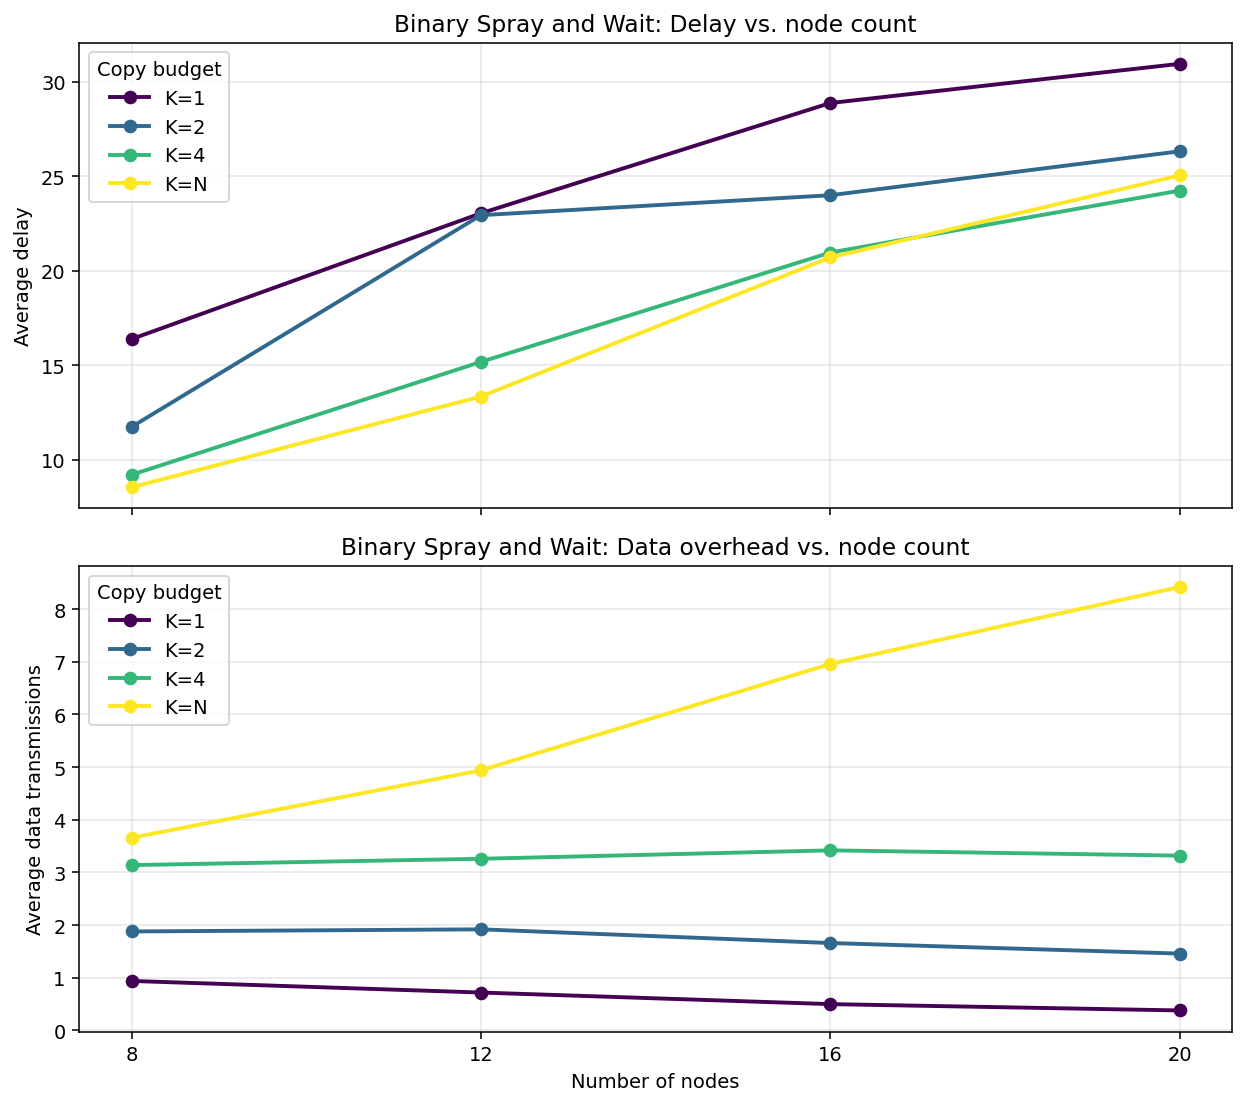
\includegraphics[width=\linewidth]{../results/spray_wait_k1_k2_k4_kn/spray_wait_metrics.png}
    \caption{Average delay and data-forwarding overhead for Binary Spray and Wait.}
    \label{fig:metrics}
\end{figure}

Figure~\ref{fig:control} explains an initially counterintuitive behavior we observed during development. If one counts all transmissions together, larger $K$ can appear cheaper because faster delivery reduces the amount of later protocol chatter. Separating control traffic reveals that this reduction comes from fewer summary exchanges rather than fewer forwarded bundle copies. In other words, larger $K$ increases \emph{data} overhead but often decreases \emph{control} overhead by shortening the time until success.

\begin{figure}[t]
    \centering
    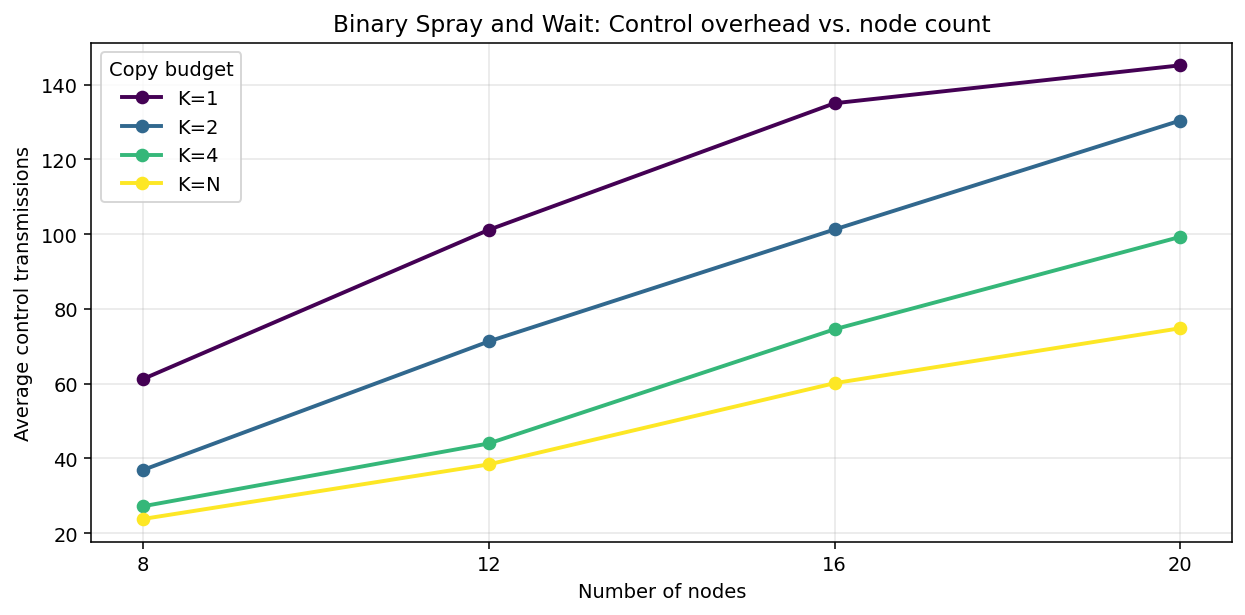
\includegraphics[width=\linewidth]{../results/spray_wait_k1_k2_k4_kn/spray_wait_control_overhead.png}
    \caption{Average control overhead measured as summary exchanges.}
    \label{fig:control}
\end{figure}

\subsection{Interpretation}

These results are consistent with the intuition behind Spray and Wait. Direct transmission ($K{=}1$) is inexpensive in terms of bundle copies, but it relies on the source or the current single holder meeting the destination directly, which becomes increasingly unlikely in larger sparse networks. Adding copies increases the chance that some carrier will meet the destination earlier, thereby improving delivery rate and often reducing delay. Binary splitting provides a disciplined version of this replication: it is far less wasteful than flooding, yet much more robust than direct delivery.

The results also show that there is no single universally optimal $K$ if one values all metrics equally. Small $K$ minimizes data transmissions but suffers poor reliability in larger networks. Large $K$ maximizes reliability but pays more in forwarding cost. This is exactly the tradeoff the protocol is designed to expose.

\subsection{Limitations}

Our evaluation is intentionally simple, and the claims of this report should be interpreted accordingly. First, the encounter model is synthetic: pairwise meetings are sampled from a Poisson process rather than from mobility traces or social-contact data. Second, the experiments involve only one outstanding bundle at a time, so there is no queueing competition, buffer pressure, or fairness issue. Third, the fixed source-destination pair is held constant across trials for each network size; only the encounter realization changes. Finally, the current implementation does not compare against a fully implemented epidemic-routing baseline in the same code path, although $K{=}1$ provides a useful direct-delivery baseline and $K{=}N$ provides an aggressive replication reference point.

Despite these limitations, the study is still credible as a compact simulator-based evaluation because the model matches the core assumptions of the protocol, the experiments are repeated many times, the metrics are carefully defined, and the conclusions are aligned with the evidence rather than overstated.
